\documentclass[11pt,compress,t,notes=noshow, aspectratio=169, xcolor=table]{beamer}

\usepackage{../../style/lmu-lecture}
% Defines macros and environments
% This file is included in slides and exercises

% Rarely used fontstyle for R packages, used only in 
% - forests/slides-forests-benchmark.tex
% - exercises/single-exercises/methods_l_1.Rnw
% - slides/cart/attic/slides_extra_trees.Rnw
\newcommand{\pkg}[1]{{\fontseries{b}\selectfont #1}}

% Spacing helpers, used often (mostly in exercises for \dlz)
\newcommand{\lz}{\vspace{0.5cm}} % vertical space (used often in slides)
\newcommand{\dlz}{\vspace{1cm}}  % double vertical space (used often in exercises, never in slides)
\newcommand{\oneliner}[1] % Oneliner for important statements, used e.g. in iml, algods
{\begin{block}{}\begin{center}\begin{Large}#1\end{Large}\end{center}\end{block}}

% Don't know if this is used or needed, remove?
% textcolor that works in mathmode
% https://tex.stackexchange.com/a/261480
% Used e.g. in forests/slides-forests-bagging.tex
% [...] \textcolor{blue}{\tfrac{1}{M}\sum^M_{m} [...]
% \makeatletter
% \renewcommand*{\@textcolor}[3]{%
%   \protect\leavevmode
%   \begingroup
%     \color#1{#2}#3%
%   \endgroup
% }
% \makeatother


\title{Interpretable Machine Learning}
\date{}

\begin{document}

	
% Set style/preamble.Rnw as parent.

% Load all R packages and set up knitr

% This file loads R packages, configures knitr options and sets preamble.Rnw as 
% parent file
% IF YOU MODIFY THIS, PLZ ALSO MODIFY setup.Rmd ACCORDINGLY...

% Defines macros and environments
\newcommand{\titlefigure}{figure/dbscan.jpg}
\newcommand{\learninggoals}{
\item Understand the aspects that undermine users' trust in an explanation
\item Learn diagnostic tools that could increase trust }

\lecturechapter{Increasing Trust in Explanations}
\lecture{Interpretable Machine Learning}

% Prerequisites: LIME and SHAP

% ------------------------------------------------------------------------------


% ------------------------------------------------------------------------------

\begin{frame}{Motivation \& Important Properties}
	\begin{itemize}
		\item Local explanations should not only make a model interpretable but also reveal if the model is trustworthy
	    \pause
	    \item \textbf{Interpretable}: ``Why did the model come up with this decision?''
	    \pause
	    \item \textbf{Trustworthy}: ``How certain is this explanation?''
	    \begin{enumerate}
	        \item accurate insights into the inner workings of our model
	        \begin{itemize}
	            \item Failure case: generation is based on inputs in areas where the model was trained with little or no training data (extrapolation)
	        \end{itemize}
	        \pause
	        \item robust (i.e. low variance)
	        \begin{itemize}
	            \item Expectation: similar explanations for similar data points with similar predictions
	            \item However, multiple sources of uncertainty exist
	            \item[$\leadsto$] measure how robust an IML method is to small changes in the input data or parameters
	            \item[$\leadsto$] Is an observation out-of-distribution?
	        \end{itemize}
	    \end{enumerate}
	    \pause
		\item Failing in one of these $\leadsto$ undermining users' trust in the explanations\\ $\leadsto$ undermining trust in the model 
		%\item In the upcoming section, we will, therefore, discuss methods to detect if a point is out-of-distribution and to measure how robust IML methods are.
	\end{itemize}
\end{frame}

\begin{frame}[c]{Out-of-distribution Detection}
	\begin{itemize}
		\item Models are unreliable in areas with little data support\\ $\leadsto$ explanations from local explanation methods are unreliable
		\pause
		\item For local explanation methods, the following components could be out-of-distribution (OOD): 
		\begin{itemize}
			\item The data for LIME's surrogate model
			\item Counterfactuals themselves
			\item Shapley value's permuted observations to calculate the marginal contributions 
			\item ICE curves grid data points 
		\end{itemize}
		\pause
		\item Two very simple and intuitive approaches
		\begin{itemize}
		    \item Classifier for out-of-distribution
		    \item Clustering
		\end{itemize}
		\item More complicated also possible, e.g., variational autoencoders [\href{https://arxiv.org/abs/1912.05651}{Daxberger et al. 2020}]
	\end{itemize}
\end{frame}


\begin{frame}[c]{Out-of-distribution Detection: OOD-Classifier}
	\begin{itemize}
	    \item Problem: we have only in-distribution data
	    \item Idea: Hallucinate new (out-of-distribution) data by randomly sample data points
	    \item[$\leadsto$] Learn a binary classifier to distinguish between the origins of the data
	    \medskip
	    \pause
	    \item Study whether an explanation approach can be fooled \citebutton{Dylan Slack et al. 2020}{https://arxiv.org/abs/1911.02508}
	    \begin{itemize}
	        \item Hide bias in the true (deployed) model, but use an unbiased model for all out-of-distribution samples
	    \end{itemize}
	    \item[$\leadsto$] Important way to diagnose an explanation approach
	\end{itemize}
\end{frame}

\begin{frame}[c]{Out-of-distribution Detection: Clustering via DBSCAN}
\begin{itemize}
	\item DBSCAN is a data clustering algorithm \citebutton{Martin Ester et al. 1996}{https://www.aaai.org/Papers/KDD/1996/KDD96-037.pdf}\\ (Density-Based Spatial Clustering of Applications with Noise) 
	\pause
	\item For this method, we define an $\epsilon$-neighborhood: \\
	Given a dataset $X = \{\xi\}_{i = 1}^n$, an $\epsilon$-neighborhood for $\xv \in \Xspace$ is defined as 
	$$ \mathcal{N}_{\epsilon}(\xv) = \{\xi \in \Xspace | d(\xv, \xi) \le \epsilon\}.$$
	 $d(\cdot)$ is a distance measure (e.g., Euclidean or Gower distance) 
	 \pause
	\item Core observations $\xv$
	\begin{itemize}
	    \item Have at least $m$ data points within $\mathcal{N}_{\epsilon}(\xv)$
	    \item Forms an own cluster with all its neighborhood points
	\end{itemize}
	\pause
    \item Border points
    \begin{itemize}
        \item Within $\mathcal{N}_{\epsilon}(\xv)$
        \item Part of a cluster defined by a core point
    \end{itemize}
    \pause
    \item Noise points
    \begin{itemize}
        \item Are not within $\mathcal{N}_{\epsilon}(\xv)$
        \item Not part of any cluster
    \end{itemize}
\end{itemize}
\end{frame}

\begin{frame}[c]{Out-of-distribution Detection}
\vspace{-0.6cm}
\begin{columns}[totalwidth=\textwidth]

	\begin{column}{0.5\textwidth}
	    \vspace{-2em}
		\begin{center}
			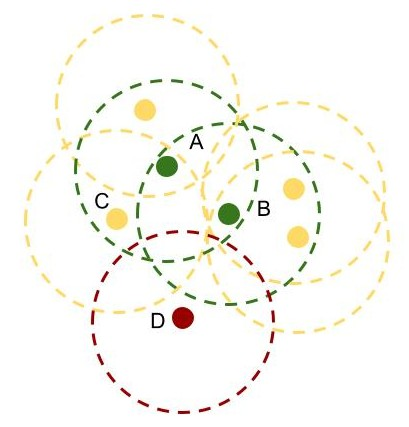
\includegraphics[width=0.6\textwidth]{figure/dbscan.jpg}\\
			\tiny{Example for DBSCAN, circles display $\epsilon$-neighborhoods, $m = 4$}
		\end{center}
	\end{column}

	\begin{column}{0.5\textwidth}
	
		\begin{itemize}
			\item Green points A and B are core points and form one cluster since they lie in each others neighborhood, all yellow points are border points of this cluster 
			\pause
			\item Since D is not part of the neighborhood of core points, it is a noise point 
			\pause
			\item In-distribution: new point lies within a cluster
			\pause
		    \item Out-of-distribution: new point lies outside the clusters 
		\end{itemize}
	\end{column}

\end{columns}

\pause

\hspace{1em}
\begin{itemize}
		\item Disadvantages:
		\begin{itemize}
		    \item Depending on the distance metric $d(\cdot)$, DBSCAN could suffer from the ``curse of dimensionality'' 
		    \item The choice of $\epsilon$ and $m$ is not clear a-priori 
		\end{itemize}
\end{itemize}
\end{frame}

\begin{frame}[c]{Robustness}
		\begin{itemize}
		\item Differentiate between different kinds of uncertainty: 
		\begin{enumerate}
			\item \textbf{Explanation uncertainty}: Change of explanation if we repeat the process, e.g., the explanation could differ depending on which subset of data we use for the explanation method and which hyperparameters 
			\pause
			\item \textbf{Process uncertainty}: Change of explanation if the underlying model is changed\\ $\leadsto$ are ML models non-robust, e.g., because they are trained on noisy data?
		\end{enumerate}
		\pause
		\item We focus on explanation uncertainty 
		\begin{itemize}
		    \item Even with the same model and same (or similar) data points, we can receive different explanations
		\end{itemize}
	\end{itemize}
\end{frame}

\begin{frame}[c]{Robustness Measure for LIME and SHAP}  
	\begin{itemize}
		\item Objective: Similar explanations for similar inputs (in a neighborhood) 
		\pause
		%\item In the previous chapter on the limitations of LIME, we already saw an example where LIME produced different explanations for very similar data points (with similar predictions).
		\item For LIME and SHAP, notion of stability based on \textbf{locally Lipschitz continuity} \citebutton{Alvarez-Melis and Jaakkola 2018}{https://arxiv.org/abs/1806.08049}:\\
		An explanation method $g:\Xspace \rightarrow \R^m$ is locally Lipschitz if 
		\begin{itemize}
		    \item for every $\xv_0 \in \Xspace$ there exist $\delta > 0$ and  $\omega \in \R$
		    \item such that $||\xv - \xv_0|| < \delta$ implies $||g(\xv) - g(\xv_0)|| < \omega ||\xv - \xv_0||$
		\end{itemize}
		\footnotesize Note that, for LIME, $g$ returns the $m$ coefficients of the surrogate model \normalsize
		\pause
		\item According to this, we can quantify the robustness of explanation models in terms of $\omega$:
		\begin{itemize}
		    \item[$\leadsto$] The closer $\omega$ is to 0, the more robust our explanation method is 
		\end{itemize}
		\pause
		\item $\omega$ is rarely known a-priori but it could be estimated as follows: 
		$$\hat{\omega}_{X}(\xv) \in \underset{\xi \in \mathcal{N}_{\epsilon}(\xv)}{\arg \max} \frac{||g(\xv) - g(\xi)||_2}{d(\xv, \xi)},$$
		where $\mathcal{N}_{\epsilon}(\xv)$ is the $\epsilon$-neighborhood of $\xv$
	\end{itemize}
\end{frame}


\begin{comment}
\begin{frame}{Sources of Uncertainty}
Two sources of uncertainty could be identified for local explanation methods: 
\begin{itemize}
\item Sampling variance in explaining a single data point. 
E.g., to train a surrogate model for LIME we sample a new data set.   
\item Sensitivity to choice of parameters. E.g., the user needs to determine the sample size and the kernel width to explain a model with LIME. 
\end{itemize}
These sources could lead to different explanations although we analyse the same model and the same (or a very similar) data point. 
\footnote[frame]{Zhang et al. (2019). ``Why Should You Trust My Explanation?'' Understanding Uncertainty in LIME Explanations. arXiv preprint arXiv:1904.12991.} 
\end{frame}
\end{comment}


\begin{comment}
\begin{frame}{Noisy data}
	\begin{itemize}
		\item What if the ML model was trained on noisy data? Should the explanation model also take up these noisy patterns? 
		\item If we use an explanation model to debug the ML model, it is okay, if our explanation model also takes up the noisy patterns learned in the ML model. 
		\item If we use an explanation model to understand both the predictor but also the underlying true data generating process, we want to focus on the stable patterns learned by the ML model and receive robust explanations. 
	\end{itemize}
\end{frame}

\begin{frame}{Addtional notes}
	\begin{itemize}
		\item We cannot only impose that the explanation of one particular method is similar for similar data points, but also across multiple IML methods. 
	\end{itemize}
\end{frame}

content...
\end{comment}

\endlecture
\end{document}
